\documentclass[11pt]{article}
\usepackage[margin=1in]{geometry}
\usepackage{volfit_preamble}
\graphicspath{{figures/}}

\title{\textbf{The Missing Derivative}\\[2pt]
\large What a surface cannot tell you: smile transport, the SSR, and the
one regime that derives its own answer\\[2pt]
\normalsize Vol-Fitter Technical Notes, No.~12}
\author{Vol-Fitter}
\date{\today}

\begin{document}
\maketitle

% Generated numbers.  ssr_derivative_tables.tex carries everything unique
% to this edition (gen_ssr_derivative.py).  Never retype a generated number.
% Auto-generated by gen_ssr_derivative.py — do not edit.
\newcommand{\smdskew}{-0.354}
\newcommand{\smdmove}{-5}
\newcommand{\smddeltagap}{19.7}
\newcommand{\smdwinggapbp}{111}
\newcommand{\smdssrshort}{2.09}
\newcommand{\smdssrlong}{2.00}
\newcommand{\smdrefagree}{\ensuremath{1.0\times10^{-17}}}
\newcommand{\smdgencommit}{40b3fa9}
\newcommand{\smdgendate}{2026-07-19}


\begin{abstract}
A calibration delivers $\sigma(k,T)$ at one spot; hedging needs
$\partial\sigma/\partial(\text{spot})$, and no snapshot contains it ---
through every arbitrage-free surface passes a family of equally
admissible tomorrows.  This lecture develops the Vol-Fitter's spot--vol
dynamics from that gap.  The missing derivative is one number per unit
of skew: requiring a first-order transport to preserve the smile's
shape leaves exactly a re-indexing plus a level, and the single free
scalar is the skew-stickiness ratio $R$ --- sticky-moneyness ($R=0$),
sticky-strike ($R=1$), sticky-local-vol ($R\approx2$) are points on one
dial, realized by a one-line transport.  The stakes are not academic:
on the live long-dated SPY smile (ATM skew $\smdskew$ per unit
log-moneyness) the regime choice moves an OTM put's delta by
\smddeltagap\ delta points --- same book, same surface.  The lecture's
second half is the regime that \emph{answers} instead of asks: freezing
the local-volatility surface in absolute strike determines the
transport exactly (the Hagan log-moneyness map, whose ATM expansion
reads the old curve two units per unit move --- the famous
$R\approx2$ is the half-rule ``implied skew is half the local skew''
in motion), diverging from the linear transport by up to
\smdwinggapbp\ vol bp in the wings on a $5\%$ move; and the exact
frozen-grid Dupire reprice, for which the SSR is an \emph{output}:
measured across maturities it runs from \smdssrshort\ at seven weeks to
\smdssrlong\ at eighteen months on a time-homogeneous surface,
hugging the theoretical short-maturity limit of $2$.  Every transport
is recalibration-free arithmetic; the one exception --- the exact
reprice --- pays one Dupire solve and is chosen explicitly.
\end{abstract}

\newpage
\tableofcontents
\newpage

%======================================================================
\section{The derivative the data does not contain}
\label{sec:missing}

A calibrated surface is a snapshot at one spot.  The next tick moves
spot, and the desk needs the new smile now --- faster than a
recalibration, and consistently with \emph{some} view of how smiles
move.  The uncomfortable fact first:

\begin{remark}[Dynamics are not identified by a snapshot]
\label{rem:ident}
Fix today's arbitrage-free surface $\sigma_0(k,T)$.  For any smooth
one-parameter family $\sigma_\eta(k,T)$ of arbitrage-free surfaces with
$\sigma_{\eta=0}=\sigma_0$, the hypothesis ``after a log-forward move
$h$ the surface is $\sigma_{\eta(h)}$'' is consistent with every price
quoted today.  Today's quotes constrain today's marginals (Notes
01--10); the derivative along spot is extra structure the desk must
\emph{choose} --- or derive from a model, which is \cref{sec:answer}.
Stochastic-volatility modelling constrains the choice (Bergomi's
short-dated bounds put one-factor models between the sticky-strike and
sticky-local-vol answers \cite{Bergomi2016}) but no static surface
selects a point.
\end{remark}

The choice has a price tag.  A vanilla's spot sensitivity is the Black
delta \emph{plus} vega times the missing derivative, so two desks
holding the same book against the same surface but different dynamics
carry different deltas.  \Cref{fig:delta} computes it on the live SPY
smile: at a representative OTM put strike the sticky-moneyness and
sticky-local-vol deltas sit \smddeltagap\ delta points apart.  The
regimes of this note are not a display preference; they are hedge
ratios.

\begin{figure}[H]
\centering
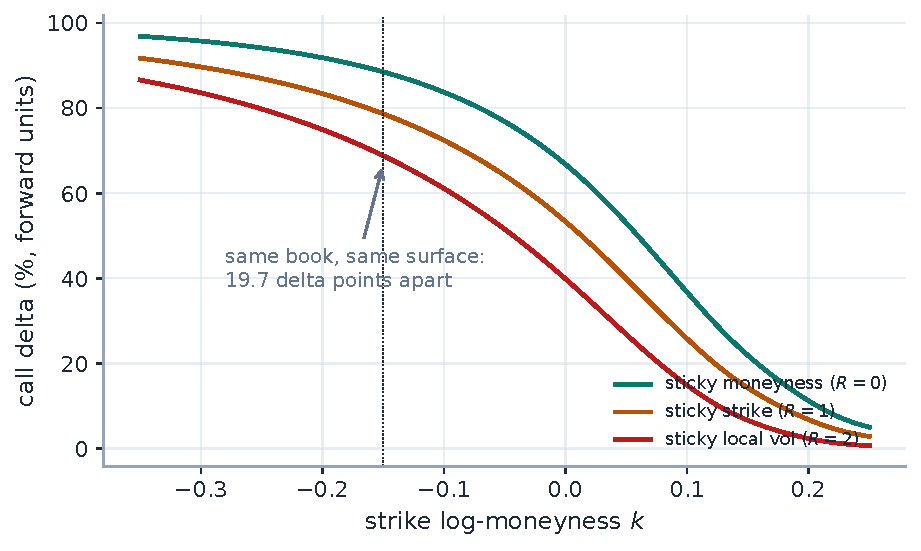
\includegraphics[width=0.86\textwidth]{fig_smd_delta.pdf}
\caption{The stakes (live SPY smile, production Black machinery,
transports finite-differenced through the production rule).  Total call
delta --- Black delta plus the smile response --- under the three
canonical regimes.  At the marked put strike the choice of dynamics is
worth \smddeltagap\ delta points on the same book against the same
surface.  Exercise~1 derives the gap as
$\mathrm{vega}\cdot(R-1)\,s_0$ per unit $R$.}
\label{fig:delta}
\end{figure}

\begin{invariant}
\begin{enumerate}[leftmargin=1.6em]
\item Every transport is recalibration-free: a spot move refreshes the
surface by arithmetic on existing objects.  The one exception --- the
exact frozen-grid reprice --- costs a single Dupire solve and is chosen
explicitly.
\item $h=0$ is the identity in every regime.
\item The three sign rules of \cref{ass:signs} are fixed once,
implemented sign-for-sign, and independently test-locked.
\item Transports wrap \emph{reads}; the calibrated anchor is never
mutated (the graph layer of Note~14 deliberately consumes the
un-transported anchor and transports its own baseline).
\end{enumerate}
\end{invariant}

\paragraph{Conventions and the notation ledger.}
$T$ is maturity; $h=\log(F_{\mathrm{new}}/F_{\mathrm{old}})$ is the one
move symbol (positive up).  Subscripted $\partial$; no primes.

\begin{table}[H]
\centering\footnotesize
\setlength{\tabcolsep}{3pt}
\begin{tabular}{@{}llll@{}}
\toprule
$k,\ K,\ F,\ h$ & log-moneyness; strike; forward; move &
$\sigma(k),\ \tvar(k,T)$ & implied vol; total variance\\[2pt]
$s_0,\ s_T$ & ATM skew $\partial_k\sigma|_{0}$ (slice; at $T$) &
$R$ & the skew-stickiness ratio (SSR)\\[2pt]
$\ell_T(k,h)$ & the exact sticky-LV displacement &
$\beta=1-\tfrac{R}{2}$ & grid barycenter weight\\
\bottomrule
\end{tabular}
\caption{Every symbol in the note.  One move symbol ($h$), one skew
symbol family ($s$); $R$ is both the ratio and the regime dial.}
\label{tab:ledger}
\end{table}

%======================================================================
\section{One free parameter}
\label{sec:oneparam}

\subsection{The sign discipline}

Every sign error in smile transport comes from mixing two coordinate
systems, so the conventions are fixed once and the code follows them
sign-for-sign.

\begin{assumption}[Sign conventions]
\label{ass:signs}
(i) The move is $h=\log(F_{\mathrm{new}}/F_{\mathrm{old}})$: positive
when the forward rises.  (ii) Log-moneyness $k=\log(K/F)$ is always
measured against the \emph{prevailing} forward --- so the same absolute
strike has \emph{lower} moneyness after an up-move:
$k_{\mathrm{new}}=k_{\mathrm{old}}-h$.  (iii) A transported
\emph{curve} is a function of new moneyness; a transported \emph{quote}
(a fixed strike) is a point whose moneyness label changes.
\end{assumption}

\begin{caution}
Convention (ii) makes curves and quotes move in \emph{opposite}
directions in $k$.  Under sticky-strike the vol at each fixed strike is
unchanged; to express the \emph{new curve} at new moneyness $k$, ask
which old strike now sits there --- the one whose old moneyness was
$k+h$.  The curve transport therefore reads \emph{forward},
$\sigma_{\mathrm{new}}(k)=\sigma_{\mathrm{old}}(k+h)$ --- a plus.  But
re-labelling an existing fixed-strike quote goes the other way: its new
moneyness is $k-h$ --- a minus.  Both signs are correct, both are in
production (the smile transport uses $k+h$; the local-vol view
re-indexes stored quotes by $k-h$), and swapping either flips the skew
response.  \Cref{fig:signs} draws both on one move; the sign-locking
tests are the fence.
\end{caution}

\begin{figure}[H]
\centering
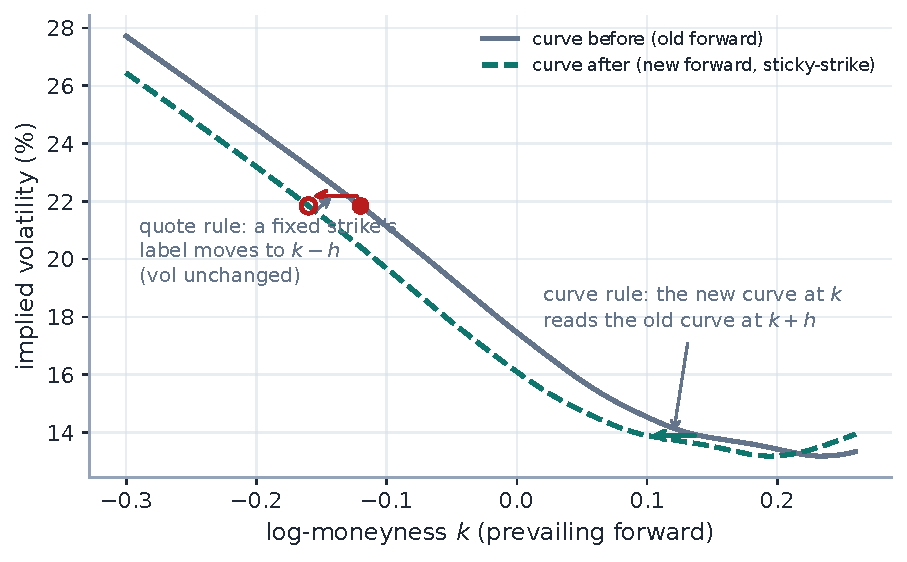
\includegraphics[width=0.86\textwidth]{fig_smd_signs.pdf}
\caption{The two signs, on one $+4\%$ move (live SPY smile,
sticky-strike).  A fixed strike keeps its vol but its \emph{label}
slides to $k-h$ (the quote rule, filled to open marker); the new curve
at any $k$ \emph{reads} the old curve at $k+h$ (the curve rule).
Opposite directions, both correct, both in production.}
\label{fig:signs}
\end{figure}

\subsection{The transport, and why it has exactly one dial}

Ask for the simplest transport consistent with
\cref{ass:signs}: built from the two operations a curve admits without
changing its shape --- a re-indexing and a level shift.  The
re-indexing is forced: expressing unchanged fixed-strike vols in new
moneyness \emph{is} $\sigma_{\mathrm{old}}(k+h)$ (the caution above),
and any other displacement would shear the smile against its own
strikes.  What remains free is one scalar --- the level --- and
parametrizing it per unit of skew-times-move gives the production
transport
\begin{equation}
\boxed{\;\sigma_{\mathrm{new}}(k)
=\sigma_{\mathrm{old}}(k+h)+(R-1)\,s_0\,h .\;}
\label{eq:shift}
\end{equation}

\begin{proposition}[ATM response; the dial is the SSR]
\label{prop:atm}
Under \eqref{eq:shift}, to first order in $h$ the ATM vol moves by
$\Delta\sigma_{\mathrm{atm}}=R\,s_0\,h$; hence
\[
R=\frac{\dd\sigma_{\mathrm{atm}}/\dd\ln F}{s_0},
\]
the skew-stickiness ratio: the fraction of the skew realized as an
ATM-vol change per unit log-spot move.
\end{proposition}

\begin{proof}
$\sigma_{\mathrm{new}}(0)=\sigma_{\mathrm{old}}(h)+(R-1)s_0h
=\sigma_{\mathrm{old}}(0)+s_0h+(R-1)s_0h+O(h^{2})$.
\end{proof}

\begin{heuristic}
Read $R$ as ``how much of the skew is real.''  The skew says lower
strikes carry higher vol.  When spot drops, does the ATM vol rise to
where the old lower-strike vol was ($R=1$, sticky-strike), not move at
all in moneyness terms ($R=0$, sticky-moneyness --- the smile rides the
forward), or \emph{overshoot} ($R\approx2$, sticky-local-vol, the
empirically common short-dated regime)?  Derman's classic taxonomy
\cite{Derman1999} named the regimes; $R$ interpolates them, and
\eqref{eq:shift} realizes any value --- named regime or custom number
--- by arithmetic.
\end{heuristic}

\Cref{fig:fan} runs the production transport on the live SPY slice: the
fan of tomorrows after a $\smdmove\%$ move, and the linear ATM
responses of slope $R\,s_0$.  The transport is one line, verified
against production to \smdrefagree\ (\cref{app:ref}):

\begin{lstlisting}[caption={The SSR smile transport \eqref{eq:shift}
(distilled from \texttt{dynamics/ssr.py}; production's last argument
accepts a named regime or a numeric $R$).},label={lst:ssr}]
def shifted_smile(k, vol_curve, atm_skew, spot_return, ssr):
    h = np.log1p(spot_return)                        # log-forward move
    return vol_curve(k + h) + (ssr - 1.0)*atm_skew*h # reindex + level
\end{lstlisting}

\begin{figure}[H]
\centering
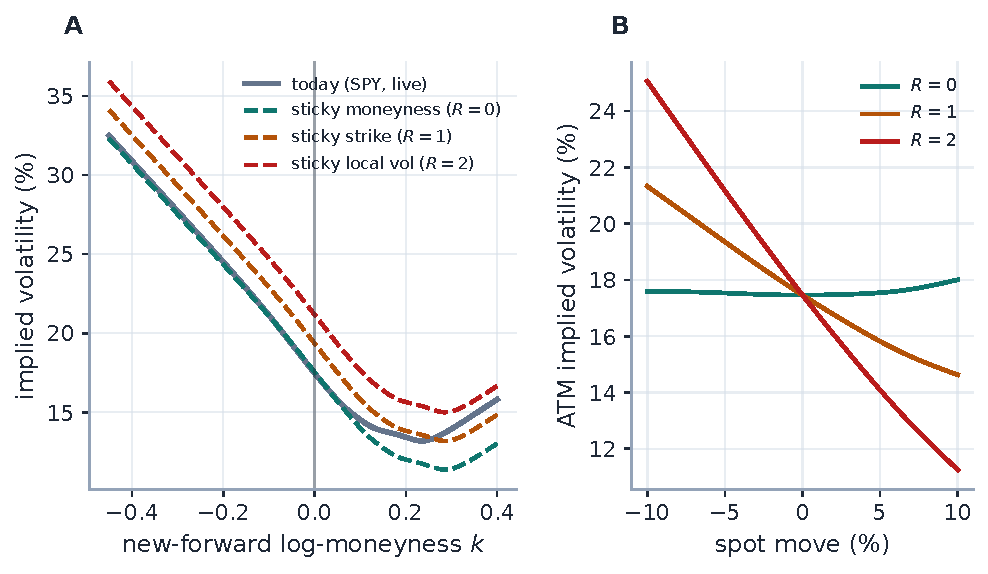
\includegraphics[width=\textwidth]{fig_smd_fan.pdf}
\caption{The fan of tomorrows (live SPY 2027-06 smile, production
transport).  A: the same surface, three regimes, one $\smdmove\%$ move
--- all three tomorrows are admissible, and today's quotes cannot
choose (\cref{rem:ident}).  B: the ATM responses are linear with slope
$R\,s_0$ (\cref{prop:atm}); the $R=0$ curve's slight bend is the
second-order term the transport does not model.}
\label{fig:fan}
\end{figure}

\paragraph{Exercise 1.}
Combine \eqref{eq:shift} with the quote rule of \cref{ass:signs} to
show a \emph{fixed strike's} vol responds as
$\dd\sigma_K/\dd\ln F=(R-1)\,s_0$ --- zero under sticky-strike, by
construction.  Hence the total delta correction is
$\mathrm{vega}\cdot(R-1)s_0$ per unit forward, and the gap between
$R=0$ and $R=2$ is $2\,\mathrm{vega}\,|s_0|$.  Evaluate it with the
Black vega at the marked strike of \cref{fig:delta} ($T=0.92$,
$\sigma\approx23\%$, $s_0=\smdskew$) and confirm the
\smddeltagap-point gap.

%======================================================================
\section{The regime that answers: frozen local volatility}
\label{sec:answer}

Every value of $R$ in \cref{sec:oneparam} is an \emph{assumption}.
There is exactly one regime in the fitter where the transport is
\emph{derived}: hold the local-volatility surface (Note~04) fixed in
absolute strike, and the new implied surface is determined --- no free
dial left.

\subsection{Why two: the half-rule}

\begin{heuristic}
For short maturities, implied vol at strike $K$ is approximately the
average of local vol along the straight path from spot to $K$ --- so
the \emph{implied} skew is about \emph{half} the local skew.  Freeze
the local curve and drop the spot by $h$: the ATM implied now averages
the local curve around the new spot, i.e.\ it slides along a curve
whose slope is $2s_0$.  The ATM response is $2\,s_0\,h$: the famous
$R\approx2$ is nothing but the half-rule read in reverse.  What the
market's skew shows is half of what the frozen generator carries, and
the motion pays out the other half.
\end{heuristic}

\subsection{The exact map}

In total-variance form the linear transport of \eqref{eq:shift} is
$\widetilde{\tvar}^{R}(T,k)=\tvar_0(T,k+R\,h)$.  The exact frozen-LV
transport replaces the linear displacement by the Hagan log-moneyness
map
\begin{equation}
\tvar^{\mathrm{LV}}(T,k)=\tvar_0\big(T,\;\ell_T(k,h)\big),
\qquad
\ell_T(k,h)=\log\!\big(e^{h}(e^{k}+1)-1\big),
\label{eq:hagan}
\end{equation}
the exact relabeling of moneyness when the local-vol surface is held
fixed in absolute strike and the forward moves by $h$
\cite{Hagan2002}.  An optional ATM re-anchor
($\sigma_{\mathrm{atm}}\to\sigma_0+R\,s_T\,h$) makes the linear SSR
response exact even for large moves.  Expanding for small $h$,
\begin{equation}
\ell_T(k,h)=k+\big(1+e^{-k}\big)h+O(h^{2}),
\qquad \ell_T(0,h)\approx 2h :
\label{eq:ellexpand}
\end{equation}
at the money the new smile reads the old curve \emph{two} units of
log-moneyness per unit move --- the half-rule's factor again, now as
the ATM slope of an exact relabeling, so $R\approx2$ is a theorem about
frozen generators, not an empirical accident.  Away from the money the
displacement $(1+e^{-k})h$ is strike-dependent --- larger on the put
wing, smaller on the call wing --- which is exactly what the linear
transport flattens into a single level adjustment.
\Cref{fig:exact} measures the price of that flattening on the live
smile: up to \smdwinggapbp\ vol bp in the wings at a $5\%$ move,
shrinking quadratically as $h\to0$ (the expansion
\eqref{eq:ellexpand} is test-locked).

\begin{figure}[H]
\centering
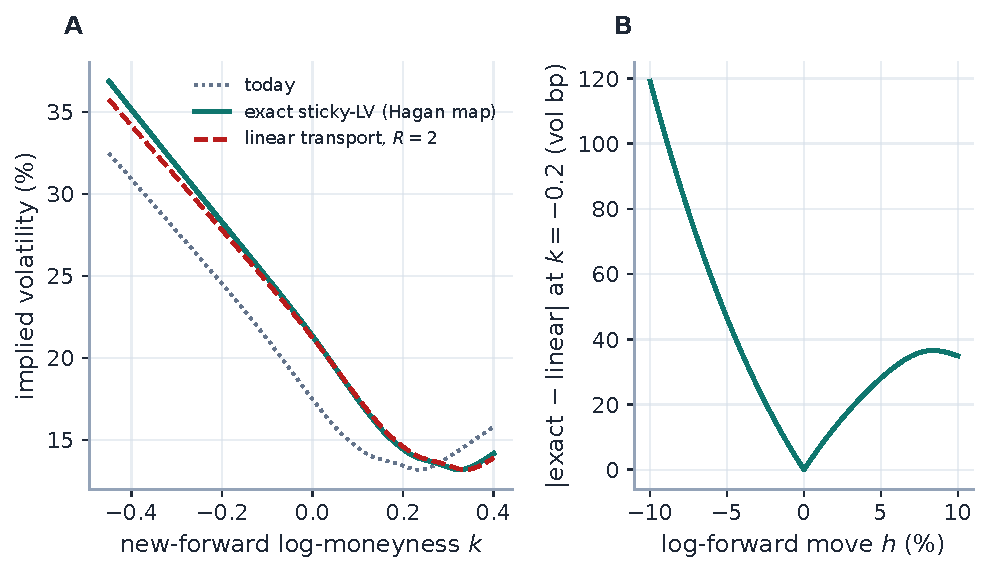
\includegraphics[width=\textwidth]{fig_smd_exact.pdf}
\caption{Exact vs linear sticky-LV (live SPY smile, production
transport both paths).  A: at a $\smdmove\%$ move the Hagan map
\eqref{eq:hagan} and the linear $R=2$ transport agree at the money and
separate in the wings --- up to \smdwinggapbp\ vol bp --- because the
exact displacement $(1+e^{-k})h$ is strike-dependent.  B: the gap at a
fixed put strike vanishes quadratically with the move: the linear
transport is exactly the first-order truncation
\eqref{eq:ellexpand}.}
\label{fig:exact}
\end{figure}

\subsection{The grid relabeling, and SSR as an output}

When the dynamics are driven by the extracted local-vol \emph{grid},
the whole taxonomy compresses into one rule for the strike nodes:
\begin{equation}
K_i \longmapsto K_i\,e^{(1-R/2)h}
\qquad\Longleftrightarrow\qquad
x_i \longmapsto x_i-\tfrac{R}{2}\,h
\quad(\text{log-moneyness nodes}),
\label{eq:gridrelabel}
\end{equation}
pinned in the tests to the exact triple $(x,\ x-\tfrac12 h,\ x-h)$ for
$R=0,1,2$.

\begin{heuristic}
Equation \eqref{eq:gridrelabel} is the cleanest statement in the note:
a stickiness regime is a rule for \emph{how the local-vol grid's
strikes follow the spot}, and $\beta=1-R/2$ is the fraction of the move
they follow --- all of it ($R=0$, the grid rides the forward), half
($R=1$), none ($R=2$, the grid frozen in absolute strike).  Everything
else --- the implied-vol shift, the ATM response, the Hagan map --- is
a consequence of that one rule.
\end{heuristic}

For $R=2$ the frozen grid can be \emph{repriced} through the Dupire PDE
rather than transported analytically --- the exact dynamics, at the
cost of one PDE solve (the note's only non-arithmetic path, selected by
its own regime name).  Here the SSR stops being an input altogether:
production reports the \emph{realized} ratio
$(\Delta\sigma_{\mathrm{atm}})/(s_0 h)$ of the reprice, and
\cref{fig:reprice} measures it across maturities on a
time-homogeneous skewed surface: \smdssrshort\ at seven weeks,
settling to \smdssrlong\ at eighteen months --- hugging the
theoretical limit $2$ of \eqref{eq:ellexpand} from above, the small
short-dated excess being the finite move and smile curvature the
first-order theory ignores.  The constant ``$2$'' in the regime table
is only this curve's limit; the reprice is the truth it approximates.

\begin{figure}[H]
\centering
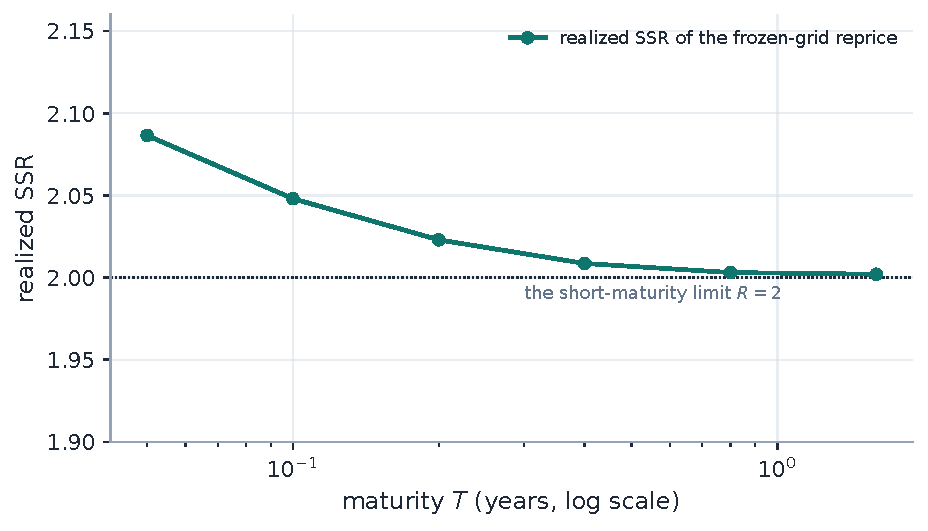
\includegraphics[width=0.82\textwidth]{fig_smd_reprice.pdf}
\caption{SSR as an output (production Dupire solver; the local-vol
grid held fixed in absolute strike, forward moved by $-2\%$, both
surfaces repriced).  The realized ratio runs from \smdssrshort\ at the
shortest maturity to \smdssrlong\ at the longest, hugging the
theoretical short-maturity limit $2$ --- measured, not assumed.}
\label{fig:reprice}
\end{figure}

\paragraph{Exercise 2.}
Derive the expansion \eqref{eq:ellexpand} from \eqref{eq:hagan}
($\partial_h\ell_T=e^{h}(e^{k}+1)/(e^{h}(e^{k}+1)-1)$, evaluate at
$h=0$).  Then evaluate the displacement at $k=\pm0.3$ for
$h=-5\%$ and explain the asymmetry of \cref{fig:exact}A: the put wing
moves $(1+e^{0.3})h\approx2.35h$ against the call wing's $1.74h$, so
the linear transport --- which spends one uniform level on both ---
errs most where the skew is steepest.

\paragraph{Exercise 3.}
Make the half-rule quantitative: for short maturities write implied
variance as the average of local variance along the chord from spot to
strike, differentiate at the money, and conclude implied skew
$=\tfrac12\times$ local skew.  Now freeze the local curve, move the
spot, and recover $R=2$.  Finally, reconcile with the measured
\smdssrshort\ at $T=0.05$ in \cref{fig:reprice}: which two ingredients
of the exact reprice does the half-rule argument drop?

%======================================================================
\section{One transport through the whole pipeline}
\label{sec:thread}

Between calibrations the transport is applied at \emph{read} time,
never to the stored fit.  A spot move wraps the cached anchor's
displayed slice in a transported view (only its total-variance function
is consulted --- the wrapper is deliberately thin), re-labels the
prepared quotes to $k-h$, and hands every consumer --- smile, term
structure, density, var-swap level, option table --- the moved smile;
the calibrated anchor itself is untouched (invariant~4).  The local-vol
workspace applies all three sign rules of \cref{ass:signs} at once, per
read: each reconstructed smile is wrapped in the curve rule, stored
fixed-strike quotes are re-indexed by the quote rule, and the shared
strike-node axis is relabelled by \eqref{eq:gridrelabel} using the
longest expiry's $h$ as the representative move.  The explicit scenario
endpoint is the one consumer of the vol-space one-liner
(\cref{lst:ssr}); its sticky-grid variant routes to the Dupire reprice
of \cref{fig:reprice} and reports the realized ratio.  A spot move
bumps a per-ticker version, so only the moved name's derived grids are
re-transported --- one name's tick never touches the rest of the
universe.

Two design decisions deserve their sentence.  First, the fitted prior
of Note~13 and the graph baseline of Note~14 are \emph{themselves}
transported: a prior calibrated at its own spot is moved to today's
forward under the active regime before it anchors or draws, so the
graph's innovation is measured against a dynamics-consistent baseline
--- and the regime choice measurably matters there (the stored graph
backtest swept $R\in\{0,1\}$: $R=0$ over-credits the graph, $R=1$
bakes the leverage effect into the baseline).  Second, the graph
universe deliberately reads the \emph{un-transported} anchor: transport
is a view, and the network's state must not depend on who looked.

\begin{remark}[The honest gap, updated]
\label{rem:gap}
The local-vol view's \emph{composite} transport (curve rule + quote
rule + grid rule applied together) still has no dedicated unit test.
Its three ingredients are each locked individually, and --- new since
the original note --- an end-to-end integration test now drives the
full composite through the API and asserts the grid relabel and
fixed-strike invariance together.  Unit-level coverage of the
composition remains the right follow-up.
\end{remark}

%======================================================================
\section{What is genuinely original here}
\label{sec:original}

The regimes are Derman's, the map is Hagan's, the SSR is Bergomi's; the
contributions are structural.
\begin{enumerate}[leftmargin=1.6em]
\item \emph{One dial, one line}: the transport \eqref{eq:shift}
realizes any SSR --- named regime or custom number --- as arithmetic on
the existing curve, with the sign discipline of \cref{ass:signs} making
the two-coordinate-system trap explicit and test-fenced.
\item \emph{The stakes made concrete}: the delta gap of
\cref{fig:delta} prices the regime choice on a live smile ---
\smddeltagap\ delta points at one strike --- turning ``display
preference'' into ``hedge ratio'' with a measured number.
\item \emph{The answering regime, graded exactly}: one parameter $R$
ties the linear shift, the Hagan map, and the frozen-grid reprice into
a speed-for-exactness ladder, with the SSR of the exact rung measured
as an output (\cref{fig:reprice}) rather than asserted as a constant
--- and the famous $2$ located precisely as that curve's short-maturity
limit.
\end{enumerate}

%======================================================================
\section{Limitations}
\label{sec:limits}

Where the guarantees stop.  \emph{The transport is first-order and
shape-frozen}: \eqref{eq:shift} moves level and label only --- no
convexity response, no vanna/volga term, and the $R=0$ panel of
\cref{fig:fan}B already shows the second-order bend it ignores.
\emph{$R$ is constant across strike and maturity} in the analytic
path; the exact reprice (whose realized $R$ does vary,
\cref{fig:reprice}) is the escape hatch, at PDE cost.  \emph{The
regime is assumed, not estimated}: nothing in the product regresses
realized ATM changes on skew to estimate the market's actual SSR ---
the dial is set by the desk (and \cref{rem:ident} is why the surface
alone cannot set it).  \emph{Large moves need the re-anchor}: the
linear ATM response degrades quadratically in $h$
(\cref{fig:exact}B); the optional re-anchor restores it exactly at the
money only.  \emph{The composite view's unit-test gap}
(\cref{rem:gap}) stands, integration coverage notwithstanding.  And
\emph{the frozen-LV answer is only as good as frozen local vol}:
empirically local vol is not invariant under spot moves --- the exact
reprice is the exact consequence of an approximate premise, which is
why it is one regime on the dial and not the dial.

\appendix
%======================================================================
\section{Hyperparameter atlas}
\label{app:atlas}

The only home for settings names: the body speaks mathematics, this
table speaks configuration.

\begin{longtable}{p{0.28\textwidth}p{0.18\textwidth}p{0.46\textwidth}}
\caption{Spot--vol-dynamics hyperparameters.}\label{tab:atlas}\\
\toprule Knob & Default & Role\\ \midrule
\endfirsthead \toprule Knob & Default & Role\\ \midrule \endhead
\texttt{dynamicsRegime} & \texttt{sticky\_strike} & Named regime
(\texttt{sticky\_moneyness} / \texttt{sticky\_strike} /
\texttt{sticky\_local\_vol} / \texttt{sticky\_local\_vol\_grid}) or
\texttt{custom}.\\
\texttt{ssr} $R$ & $2.0$ & Numeric SSR, consumed only when
\texttt{dynamicsRegime} is \texttt{custom}.\\
$R$ regime map & $\{0,1,2,2\}$ & SSR of the four named regimes; the
grid regime's $2$ is only the short-maturity limit of its reprice
(\cref{fig:reprice}).\\
ATM re-anchor & off & Optional exact linear SSR for large moves
($\sigma_0+R\,s_T\,h$).\\
\bottomrule
\end{longtable}

\noindent\textbf{Performance.}  The transport \eqref{eq:shift} and the
grid relabeling \eqref{eq:gridrelabel} are $O(\text{grid})$ arithmetic
--- no optimization, no PDE --- so a spot move refreshes the whole
surface essentially for free.  Only the exact frozen-grid reprice costs
a Dupire solve, chosen explicitly by its regime name.  A spot move
bumps the per-ticker spot version, so only the moved name's derived
grid is re-transported; the global spot version is deliberately
\emph{not} in the fit-cache key, so anchors stay warm.

%======================================================================
\section{Traceability}
\label{app:trace}

\begingroup
\small
\setlength{\tabcolsep}{4pt}
\renewcommand{\arraystretch}{1.15}
\begin{longtable}{@{}p{0.42\textwidth}p{0.10\textwidth}p{0.44\textwidth}@{}}
\caption{Claims in this note and the code/tests that lock them.}
\label{tab:trace}\\
\toprule Claim & Object & Code anchor \newline \emph{Test anchor}\\ \midrule
\endfirsthead
\toprule Claim & Object & Code anchor \newline \emph{Test anchor}\\ \midrule
\endhead
ATM moves by $R\,s_0\,h$; shape preserved &
\cref{prop:atm} &
\nolinkurl{volfit/dynamics/ssr.py}\newline
\nolinkurl{tests/test_dynamics.py::test_atm_vol_moves_by_ssr_times_skew};
\nolinkurl{::test_shape_is_preserved_up_to_level}\\
\addlinespace
$h=0$ is the identity in every regime &
invariant~2 &
\nolinkurl{volfit/dynamics/transport.py}\newline
\nolinkurl{tests/test_spot_transport.py::test_h_zero_is_identity_all_regimes}\\
\addlinespace
Sticky-moneyness / sticky-strike signs &
\eqref{eq:shift} &
\nolinkurl{volfit/dynamics/transport.py}\newline
\nolinkurl{tests/test_spot_transport.py::test_sticky_moneyness_leaves_smile_in_moneyness_unchanged};
\nolinkurl{::test_sticky_strike_fixes_vol_at_fixed_strike}\\
\addlinespace
Hagan-map expansion; double-skew ATM response &
\eqref{eq:hagan}, \eqref{eq:ellexpand} &
\nolinkurl{volfit/dynamics/transport.py}\newline
\nolinkurl{tests/test_spot_transport.py::test_ell_T_small_move_expansion};
\nolinkurl{::test_sticky_local_vol_double_skew_atm_response}\\
\addlinespace
Grid rule pinned to $(x,\,x-\tfrac12 h,\,x-h)$; $\beta=1-R/2$ &
\eqref{eq:gridrelabel} &
\nolinkurl{volfit/dynamics/transport.py}\newline
\nolinkurl{tests/test_spot_transport.py::test_grid_node_rule_barycenter};
\nolinkurl{::test_beta_of_canonical_values}\\
\addlinespace
ATM re-anchor hits the exact linear target; transported slice wraps
only the variance function &
\cref{sec:answer} &
\nolinkurl{volfit/dynamics/transport.py}\newline
\nolinkurl{tests/test_spot_transport.py::test_atm_anchor_hits_exact_linear_ssr_target};
\nolinkurl{::test_transported_slice_matches_function_and_vol}\\
\addlinespace
Frozen-grid reprice: ATM consistency and realized SSR reported &
\cref{fig:reprice} &
\nolinkurl{volfit/api/localvol.py}\newline
\nolinkurl{tests/test_api_localvol.py::test_reprice_matches_fitted_atm};
\nolinkurl{::test_sticky_grid_scenario_realized_ssr}\\
\addlinespace
Composite LV view transports without refit (integration) &
\cref{rem:gap} &
\nolinkurl{volfit/api/affine_transport.py}\newline
\nolinkurl{tests/test_spot_move_service.py::test_affine_lv_surface_transports_without_refit}\\
\addlinespace
Graph baseline transported under the active regime &
\cref{sec:thread} &
\nolinkurl{volfit/api/prior_transport.py}\newline
\nolinkurl{tests/test_api_graph.py} ($R=0\Rightarrow$ ATM shift second
order)\\
\bottomrule
\end{longtable}
\endgroup

%======================================================================
\section{Reference implementation}
\label{app:ref}

\Cref{lst:ssr} was executed against the production transport by this
edition's generator on every run --- four move/regime pairs including a
custom numeric $R$ --- agreeing to \smdrefagree\ (floating-point
identity).  The exact-path figures consume the production
total-variance transport directly (the Hagan branch for the named
local-vol regime, the linear branch for numeric $R$ --- the production
dispatch rule); the reprice figure drives the production Dupire solver
on the frozen and moved grids, never a re-implementation.

\begin{thebibliography}{9}
\bibitem{Derman1999} E.~Derman.  Regimes of volatility.
\emph{Risk}, April 1999.
\bibitem{Bergomi2016} L.~Bergomi.  \emph{Stochastic Volatility
Modeling}.  CRC Press, 2016.
\bibitem{Hagan2002} P.~Hagan, D.~Kumar, A.~Lesniewski and
D.~Woodward.  Managing smile risk.  \emph{Wilmott Magazine}, 2002.
\bibitem{Gatheral2006} J.~Gatheral.  \emph{The Volatility Surface}.
Wiley, 2006.
\end{thebibliography}

\end{document}
